% Feynman rules of a dS graph: the bubble input example of the documentation.
\documentclass[tikz,border=6pt]{standalone}
\usepackage{bm}
\usetikzlibrary{calc}
\begin{document}
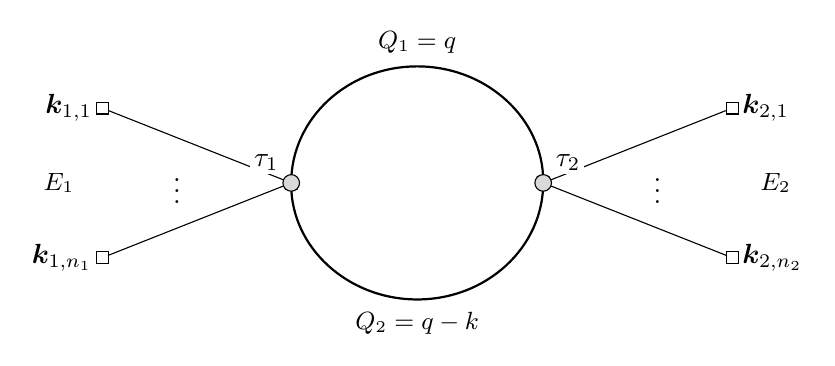
\begin{tikzpicture}[scale=1.0, every node/.style={inner sep=1.5pt}]
  \coordinate (vL) at (0,0);
  \coordinate (vR) at (3.2,0);
  \coordinate (lU) at (-2.4,0.95);
  \coordinate (lD) at (-2.4,-0.95);
  \coordinate (rU) at (5.6,0.95);
  \coordinate (rD) at (5.6,-0.95);
  \draw (vL) -- (lU) node[left=2pt] {$\bm{k}_{1,1}$};
  \draw (vL) -- (lD) node[left=2pt] {$\bm{k}_{1,n_1}$};
  \draw (vR) -- (rU) node[right=2pt] {$\bm{k}_{2,1}$};
  \draw (vR) -- (rD) node[right=2pt] {$\bm{k}_{2,n_2}$};
  \node[fill=white,inner sep=1pt] at (-1.45,0) {$\vdots$};
  \node[fill=white,inner sep=1pt] at (4.65,0) {$\vdots$};
  \draw[->,thick] (vL) arc[start angle=180,end angle=0,x radius=1.6,y radius=1.48];
  \draw[->,thick] (vR) arc[start angle=0,end angle=-180,x radius=1.6,y radius=1.48];
  \node[fill=white] at (1.6,1.78) {\small $Q_1=q$};
  \node[fill=white] at (1.6,-1.78) {\small $Q_2=q-k$};
  \node[fill=white] at (-2.95,0) {\small $E_1$};
  \node[fill=white] at (6.15,0) {\small $E_2$};
  \filldraw[fill=gray!30,draw=black] (vL) circle (3pt);
  \filldraw[fill=gray!30,draw=black] (vR) circle (3pt);
  \node[fill=white,anchor=south east] at (-0.10,0.10) {$\tau_1$};
  \node[fill=white,anchor=south west] at (3.30,0.10) {$\tau_2$};
  \filldraw[fill=white,draw=black] ($(lU)+(-0.075,0.075)$) rectangle ++(0.15,-0.15);
  \filldraw[fill=white,draw=black] ($(lD)+(-0.075,0.075)$) rectangle ++(0.15,-0.15);
  \filldraw[fill=white,draw=black] ($(rU)+(-0.075,0.075)$) rectangle ++(0.15,-0.15);
  \filldraw[fill=white,draw=black] ($(rD)+(-0.075,0.075)$) rectangle ++(0.15,-0.15);
\end{tikzpicture}
\end{document}
